\documentclass{beamer}
\usepackage[frenchb]{babel}
\usepackage[utf8]{inputenc}
\usepackage[T1]{fontenc}
\usepackage{graphicx}
\usepackage{listings}
\usepackage{color}

\definecolor{mygreen}{rgb}{0,0.6,0}
\definecolor{mygray}{rgb}{0.5,0.5,0.5}
\definecolor{mymauve}{rgb}{0.58,0,0.82}

\lstset{ %
  backgroundcolor=\color{white},   % choose the background color; you must add \usepackage{color} or \usepackage{xcolor}
  basicstyle=\tiny,        % the size of the fonts that are used for the code
  breakatwhitespace=false,         % sets if automatic breaks should only happen at whitespace
  breaklines=true,                 % sets automatic line breaking
  captionpos=b,                    % sets the caption-position to bottom
  commentstyle=\color{mygreen},    % comment style
  deletekeywords={...},            % if you want to delete keywords from the given language
  escapeinside={\%*}{*)},          % if you want to add LaTeX within your code
  extendedchars=true,              % lets you use non-ASCII characters; for 8-bits encodings only, does not work with UTF-8
  frame=none,	                   % adds a frame around the code
  keepspaces=true,                 % keeps spaces in text, useful for keeping indentation of code (possibly needs columns=flexible)
  keywordstyle=\color{blue},       % keyword style
  language=Octave,                 % the language of the code
  otherkeywords={*,...},           % if you want to add more keywords to the set
  numbers=left,                    % where to put the line-numbers; possible values are (none, left, right)
  numbersep=5pt,                   % how far the line-numbers are from the code
  numberstyle=\tiny\color{mygray}, % the style that is used for the line-numbers
  rulecolor=\color{black},         % if not set, the frame-color may be changed on line-breaks within not-black text (e.g. comments (green here))
  showspaces=false,                % show spaces everywhere adding particular underscores; it overrides 'showstringspaces'
  showstringspaces=false,          % underline spaces within strings only
  showtabs=false,                  % show tabs within strings adding particular underscores
  stepnumber=1,                    % the step between two line-numbers. If it's 1, each line will be numbered
  stringstyle=\color{mymauve},     % string literal style
  tabsize=2,	                   % sets default tabsize to 2 spaces
  title=\lstname                   % show the filename of files included with \lstinputlisting; also try caption instead of title
}

\usetheme{ENSLyon} 

\title[Adaptation de micro-architectures hétérogènes]{Adaptation de micro-architectures hétérogènes via l'utilisation de gem5 et CERE}
\author[N. Derumigny et P.De Oliveira]{Nicolas Derumigny \and Pablo de Oliveira Castro}
\institute[]{ENS Lyon \hspace*{8em} UVSQ \hspace*{3em}}
\date{5 Septembre 2016}


\usecolortheme{ENSLyon_blue}



\begin{document}



\begin{frame}
	\titlepage
	\begin{center}
	\end{center}
\end{frame}




\section{Introduction}
\begin{frame}
\begin{itemize}
\item Utilisation de morceaux de codes via CERE\cite{CERE}
\bigskip
\item Simulation de différents CPU via gem5\cite{gem5-sim}
\bigskip
\item Simulation de la consommation énergétique via McPAT\cite{McPAT}
\bigskip
\item Calcul du ratio performance-consommation énergétique
\end{itemize}
\end{frame}

\section{Outils utilisés}
\subsection{CERE}
\begin{frame}{Codelet Extractor and REplayer : Définitions}
CERE extrait des morceaux de code d'une application, créant ainsi une autre application autonome, reproduisant au plus près possible son exécution, autant dans ses instructions que dans son contexte.

\begin{block}{Codelet}
\begin{itemize}
\item Portion d'un application. 
\item \textit{In-vivo} : fonctionnement naturel à l'intérieur de son application.
\item \textit{In-vitro} : fonctionnement dans l'application produite par CERE.
\end{itemize}
\end{block}
\end{frame}

\begin{frame}{CERE : Un outil d'isolation de morceaux de code}
\begin{figure}[ht]
\begin{center}
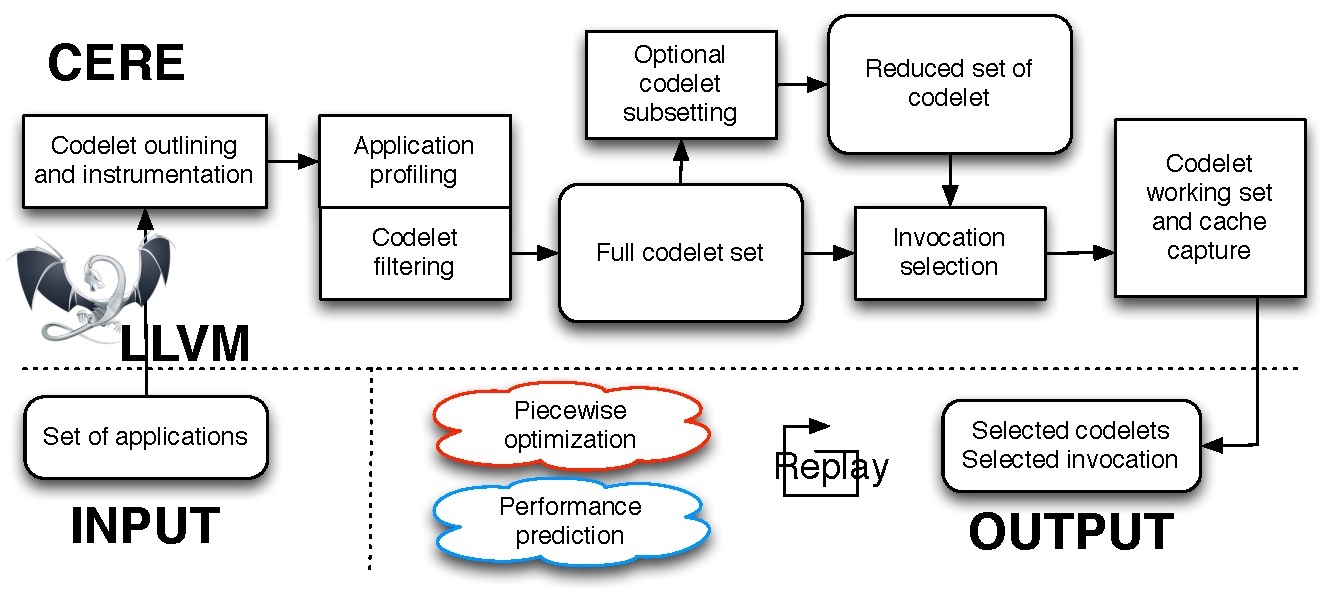
\includegraphics[width=0.85\linewidth]{cere_fonction.pdf}
\caption{\label{CERE_schema}Schéma fonctionnel de CERE.}
\end{center}
\end{figure}
\end{frame}

\subsection{Gem5}
\subsubsection{Généralités}
\begin{frame}{Gem5 : Un simulateur précis au cycle près}

\begin{itemize}
\item Projet open-source, codé en C++
\medskip
\item Utilisation de python pour le choix des configurations
\medskip
\item Support des jeux d'instruction ARM, x86, Alpha, SPARC, POWER et MIPS
\medskip
\item Simulation du fonctionnement du CPU cycle par cycle
\medskip
\item Simulation de systèmes hétérogènes
\medskip
\item Accès aux données non mesurables d'un CPU standard (cache miss) 
\end{itemize}

\end{frame}

\subsubsection{Mode d'émulation des appels systèmes}
\begin{frame}{Gem5 : Le mode \textit{syscall emulation} (SE)}
\begin{itemize}
\item Émulation d'une application au sein d'un système linux complet virtuel
\medskip
\item Besoin de codage séparé de tous les appels systèmes
\medskip
\item Pas de support des libraires dynamiques
\medskip
\item Systèmes multi-cœurs peu flexible (m5thread)
\medskip
\item Exécution d'une seule application
\end{itemize}
\end{frame}


\subsubsection{Mode d'émulation d'un système complet}
\begin{frame}{Gem5 : Le mode \textit{fullsystem} (FS)}
\begin{itemize}
\item Émulation d'un CPU "nu"
\medskip
\item Exécution d'un système linux complet par le CPU simulé
\medskip
\item Support des libraires dynamiques et des systèmes multi-cœurs via le noyau linux
\medskip
\item Exécution d'une suite quelconque de commandes
\medskip
\item Plus lent que le mode SE
\medskip
\item Nécessite au préalable la préparation d'une image disque
\end{itemize}
\end{frame}


\subsection{McPAT}
\begin{frame}{McPAT : Un simulateur de conception et de consommation de puces}
\begin{figure}[ht]
\begin{center}
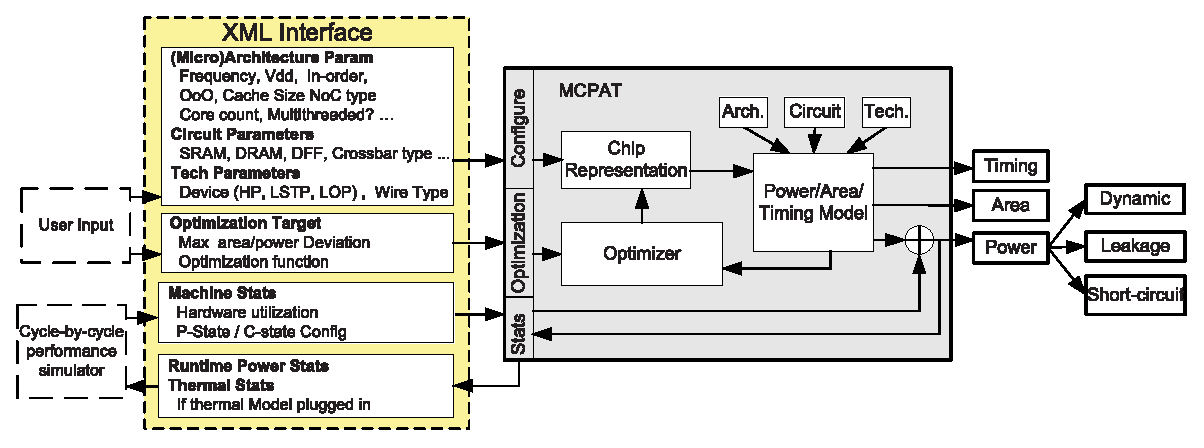
\includegraphics[width=0.84\paperwidth]{McPAT_diag.eps}
\caption{\label{McPAT_schema}Schema fonctionnel de McPAT.}
\end{center}
\end{figure}
\end{frame}


\section{Protocole de simulation}
\subsection{Patch de gem5}
\begin{frame}[fragile]{Correction de \textit{readFunc()}}
\begin{lstlisting}[language=c++]
SyscallReturn
readFunc(SyscallDesc *desc, int num, LiveProcess *p, ThreadContext *tc)
{
    int index = 0;
    int tgt_fd = p->getSyscallArg(tc, index);
    Addr bufPtr = p->getSyscallArg(tc, index);
    int nbytes = p->getSyscallArg(tc, index);
    BufferArg bufArg(bufPtr, nbytes);

    int sim_fd = p->getSimFD(tgt_fd);
    if (sim_fd < 0)
        return -EBADF;

    int bytes_read = read(sim_fd, bufArg.bufferPtr(), nbytes);

    if (bytes_read %*\textcolor{red}{> 0}*))
        bufArg.copyOut(tc->getMemProxy());

    return bytes_read;
}
\end{lstlisting}
\end{frame}

\begin{frame}[fragile]{Ajout des appels système \textit{getdents()} et \textit{getdents64()}}
\tiny
\begin{lstlisting}[language=c++]
SyscallReturn
getdentsFunc(SyscallDesc *desc, int num, LiveProcess *p, ThreadContext *tc)
{
    int index = 0;
    int sim_fd = p->sim_fd(p->getSyscallArg(tc, index));
    if (sim_fd < 0)
        return -EBADF;
    Addr buf_ptr = p->getSyscallArg(tc, index);
    int nbytes = p->getSyscallArg(tc, index);
    BufferArg buf_arg(buf_ptr, nbytes);

    int nread = syscall(SYS_getdents, sim_fd, buf_arg.bufferPtr(), nbytes);
    int errno_after_call=errno;

    if (nread > 0)
        buf_arg.copyOut(tc->getMemProxy());

    return (nread == -1) ? -errno_after_call : nread;
}
\end{lstlisting}

\end{frame}

\subsection{Configuration simulées}
\begin{frame}{Simulation de quatre processeurs aux caractéristiques diverses}
\begin{figure}[ht]
\begin{center}

\begin{tabular}{| l | c | c | c | c | c | c |}
\hline 
& & & \multicolumn{2}{c|}{L2} &\\
Nom & Fréquence & Assoc. & Taille & Assoc. & L3 \\
\hline

A15 & 1 GHz & 2 & 1 Mo & 16 & Non \\

i5-3550 & 3,3-3,7 GHz & 8 & 256 ko & 8 & 8 Mo / 16\\

i5-3337U & 1,8 GHz & 8 & 256 ko & 16 & 4 Mo / 8\\

Q9100 & 2,26 GHz & 8 & 8 Mo & 16 & Non\\
\hline

\end{tabular}
\caption{\label{cpu_setup}Paramètres utilisés pour chaque CPU. Le reste de la configuration est fixe : 8 Go de RAM, processeur x86 générique gravé en 44nm, et un unique cœur simulé.}
\end{center}
\end{figure}
\end{frame}

\subsection{Codelets choisis}
\begin{frame}{Trois codelets sur le banc d'essai}
\begin{itemize}
\item NAS IS séquentiel : région \_\_cere\_\_is\_ranked\_475, qui vérifie si un tableau est bien trié.
\item PARSEC blackscholes : région \\ \_\_cere\_\_blackscholes\_m4\_\_Z9bs\_threadPv\_first, une région parallèle OpenMP calculant la valeur d'une option en se basant sur l'équation de Black \& Scholes.
\item PARSEC freqmine : région\\ \_\_cere\_\_tree8scan1\_DBEP4Data\_first, générant un hash à partir d'un arbre de données.
\end{itemize}
\end{frame}

\section{Résultats}

\subsection{NAS IS}
\begin{frame}{IS : Une première application simple}

\begin{columns}

\begin{column}{0.4\paperwidth}
\begin{figure}
\centering
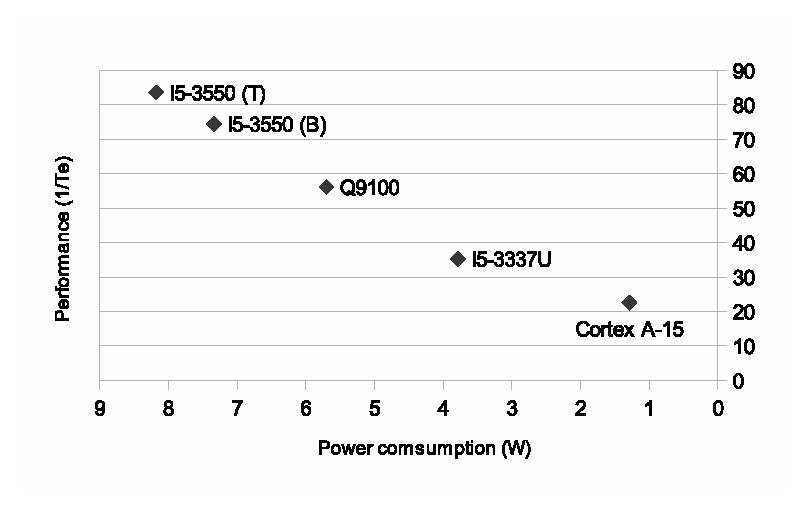
\includegraphics[width=\textwidth]{IS.eps}
\caption{\label{IS}Graphique du ratio performance-consommation énergétique du codelet \textit{IS}.}
\end{figure}
\end{column}

\begin{column}{0.4\paperwidth}
\begin{figure}
\centering
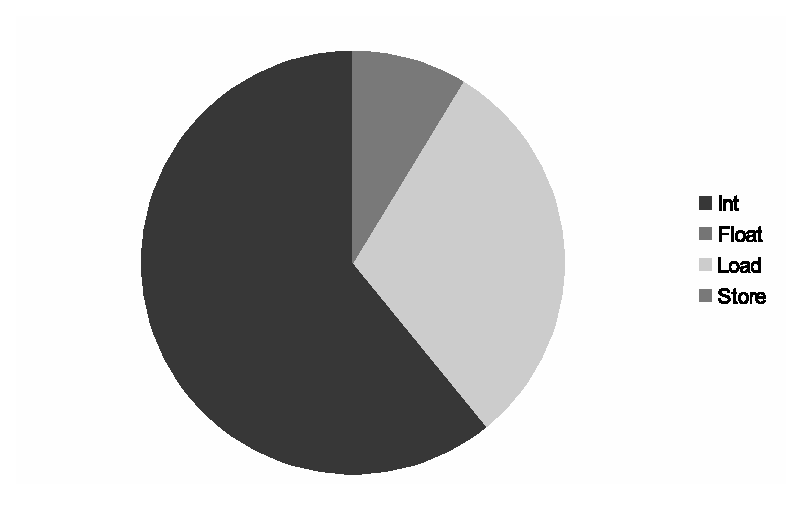
\includegraphics[width=\textwidth]{IS_instr.eps}
\caption{\label{IS_instr}Répartition des instructions au cours de l'exécution du codelet \textit{IS}.}
\end{figure}
\end{column}

\end{columns}

\end{frame}


\subsection{Freqmine}
\begin{frame}{Freqmine : Une application parallèle à peu de données}

\begin{columns}

\begin{column}{0.4\paperwidth}
\begin{figure}
\centering
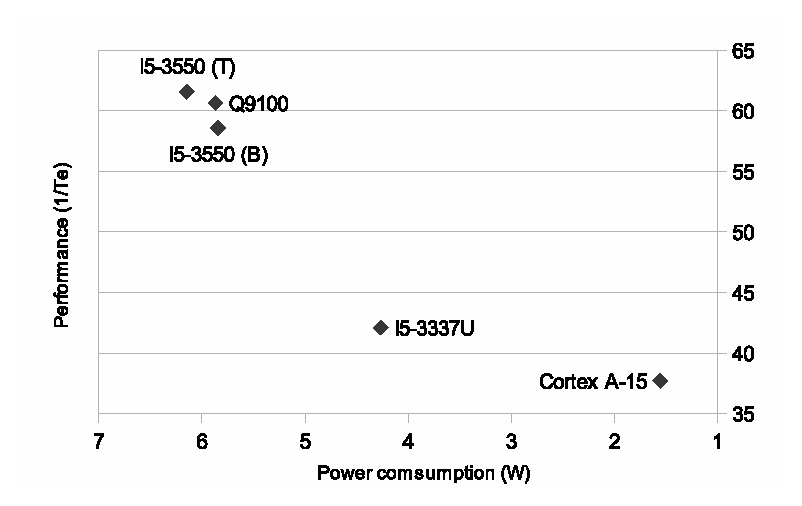
\includegraphics[width=\textwidth]{Freqmine.eps}
\caption{\label{Freq}Graphique du ratio performance-consommation énergétique du codelet \textit{Freqmine}.}
\end{figure}
\end{column}

\begin{column}{0.4\paperwidth}
\begin{figure}
\centering
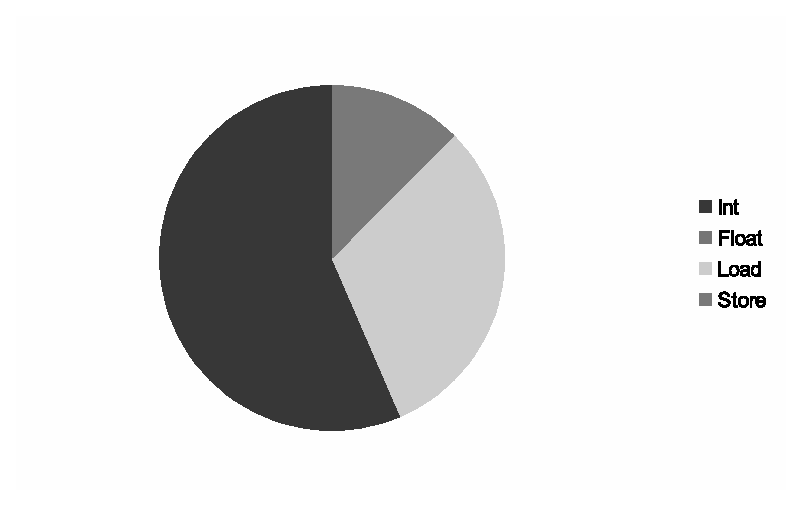
\includegraphics[width=\textwidth]{Freqmine_instr.eps}
\caption{\label{Freq_instr}Répartition des instructions au cours de l'exécution du codelet \textit{Freqmine}.}
\end{figure}
\end{column}

\end{columns}

\end{frame}

\subsection{Blackscholes}
\begin{frame}{Blackscholes : Une application utilisant significativement les flottants}

\begin{columns}

\begin{column}{0.4\paperwidth}
\begin{figure}
\centering
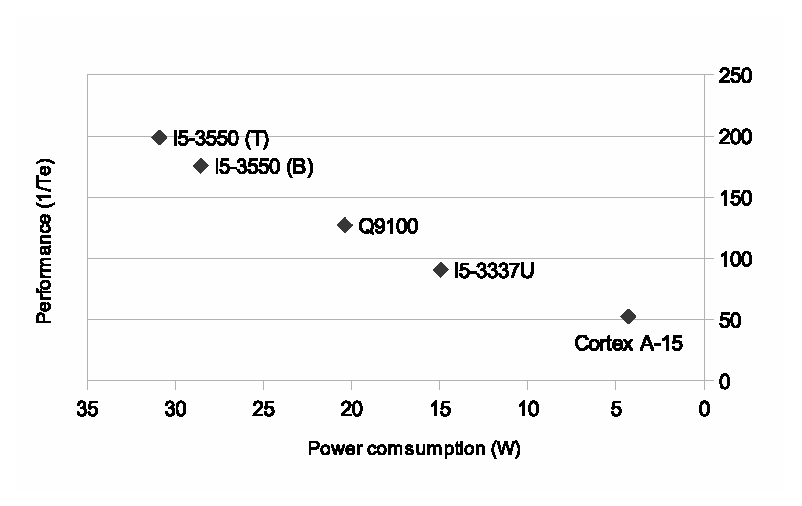
\includegraphics[width=\textwidth]{Blackscholes.eps}
\caption{\label{Blackscholes}Graphique du ratio performance-consommation du codelet \textit{Blackscholes}.}
\end{figure}
\end{column}

\begin{column}{0.4\paperwidth}
\begin{figure}
\centering
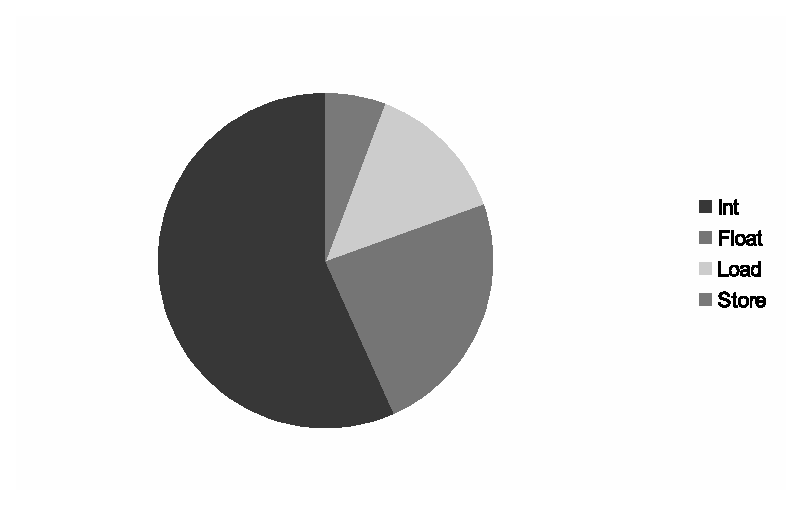
\includegraphics[width=\textwidth]{Blackscholes_instr.eps}
\caption{\label{Blackscholes_instr}Répartition des instructions au cours de l'exécution du codelet \textit{Blackscholes}.}
\end{figure}
\end{column}

\end{columns}

\end{frame}

\begin{frame}{Définition du ratio performance-consommation énergétique}
\begin{block}{Ratio performance-consommation énergétique}
Le ratio performance-consommation énergétique I est défini par :
\begin{equation*}
I=\frac{1}{P.t_e}
\end{equation*}
Avec $P$ la puissance (en W) du processeur simulé et $t_e$ le temps d'exécution du codelet (en s).
\end{block}
\textit{Note :} Cela correspond à l'inverse de la consommation totale du processeur.
\end{frame}

\subsection{Résultats généraux}

\begin{frame}{Graphe récapitulatif}
\begin{figure}
\centering
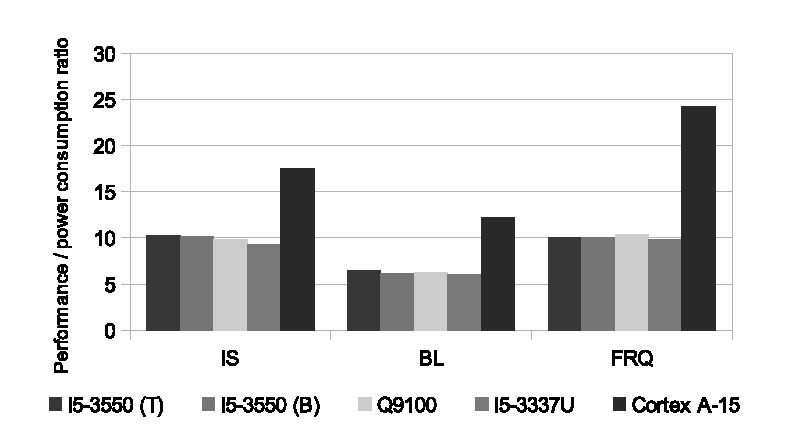
\includegraphics[width=0.65\paperwidth]{Ratio.eps}
\caption{\label{Ratio}Ratio performance-consommation énergétique pour chaque codelet.}
\end{figure}

\end{frame}

\section{Conclusion}
\begin{frame}
\begin{itemize}
\item Des résultats cohérents
\bigskip
\item Des performances plutôt indépendantes du jeu d'instruction
\bigskip
\item Influence importante de la taille du cache, parfois plus que la puissance de calcul brute
\bigskip
\item Gain de temps induit par l'utilisation de codelets
\bigskip
\item Utilisation possible comme étalon d'un ordonnanceur sur une plateforme hétérogène
\end{itemize}
\end{frame}

\section{Bibliographie}
\begin{frame}{Bibliographie}

\tiny
\bibliographystyle{plain}
\bibliography{report}
\end{frame}

\section{Annexe}
\begin{frame}{Compilation croisée depuis l'architecture x86 vers Aaarch64}

\begin{columns}

\begin{column}{0.4\paperwidth}
\begin{itemize}
\item Installation du cross-compilateur LLVM
\item Modification de CERE : compilateur linker et objdump utilisé
\item Changement de l'adresse de départ de l'exécutable
\item Changement d'adresse de la pile (cf figure)
\end{itemize}
\end{column}


\begin{column}{0.4\paperwidth}
\begin{figure}
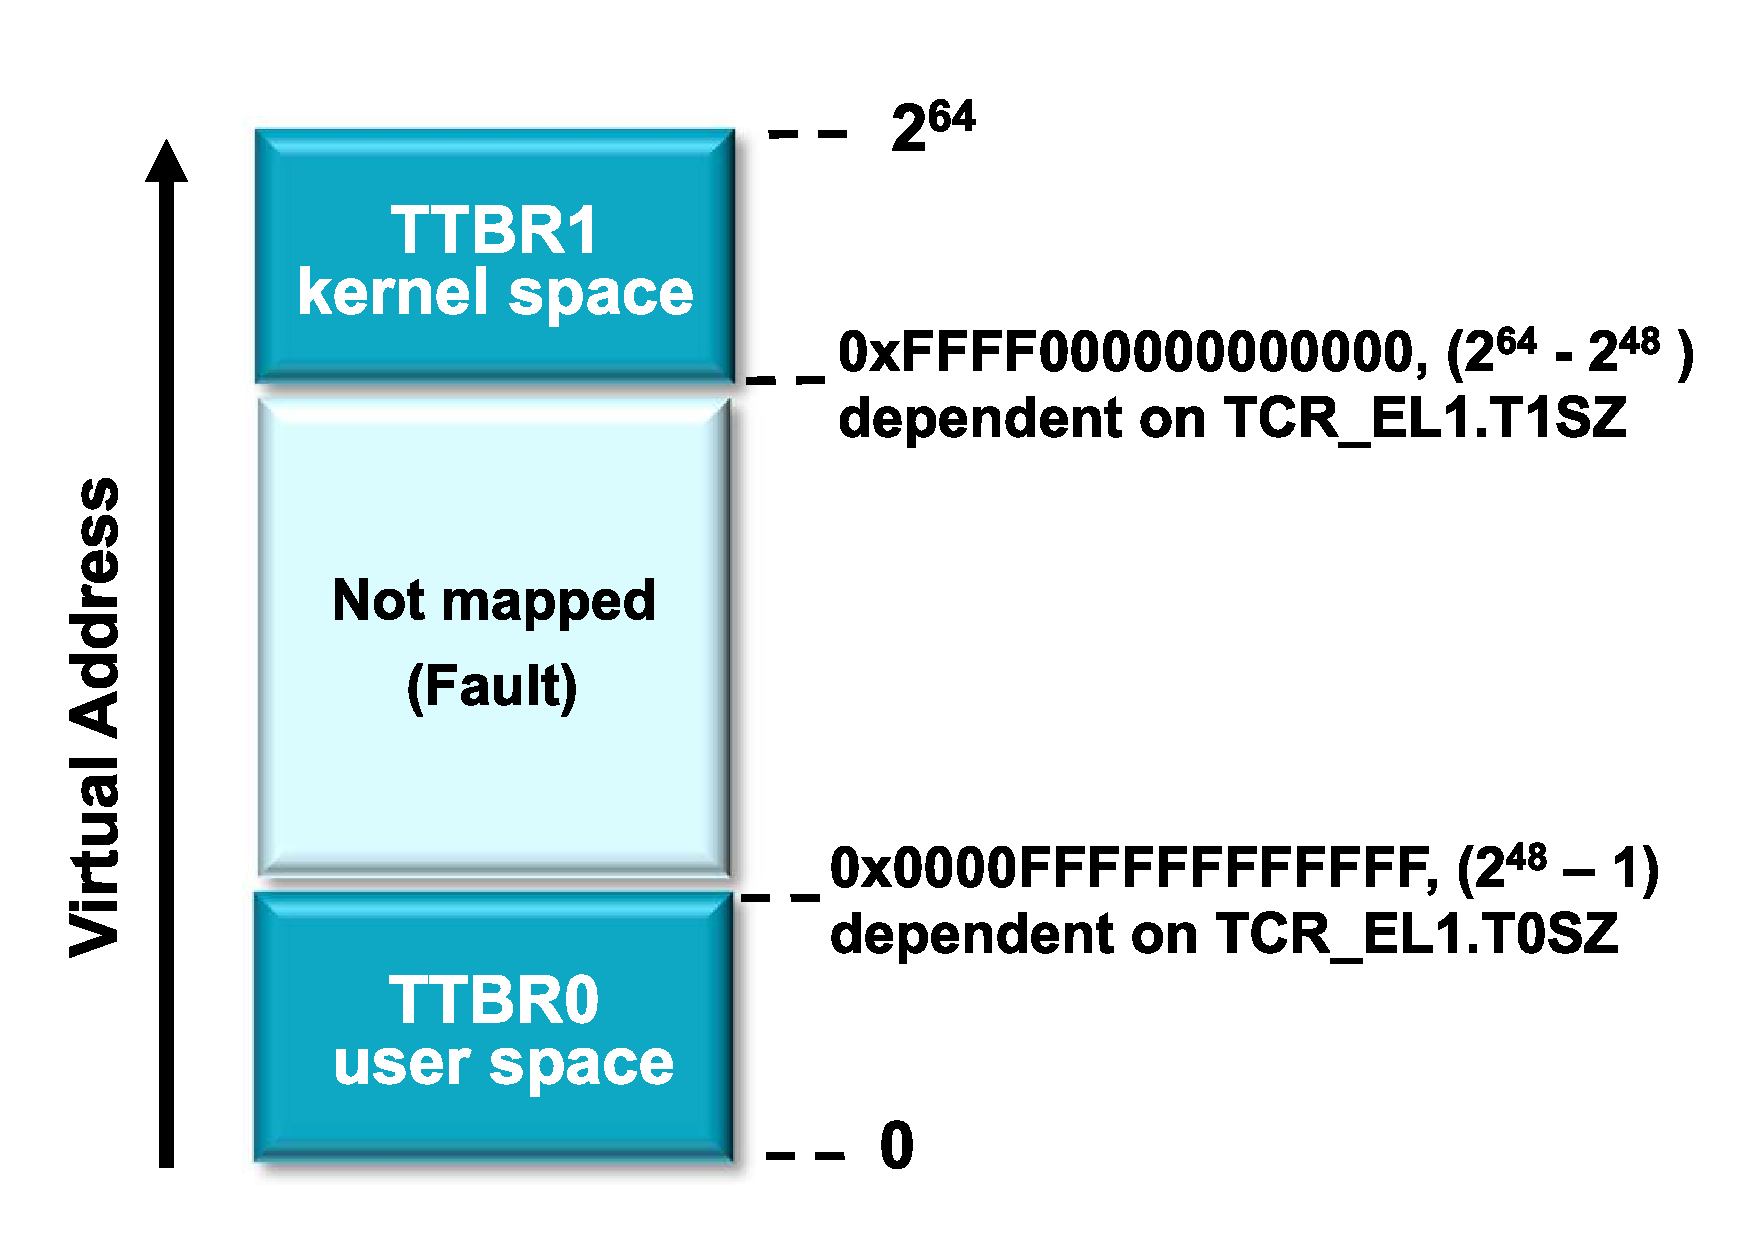
\includegraphics[width=\textwidth]{virtual_mem_aarch64.pdf}
\caption{Mappage de la mémoire virtuelle de l'architecture aarch64}
\end{figure}
\end{column}

\end{columns}

\end{frame}


\end{document}
